\documentclass[a4paper,12pt]{article}
\usepackage{geometry}
\geometry{a4paper, left=2cm, right=2cm, top=2cm, bottom=2cm}
\usepackage[utf8]{inputenc}
\usepackage[french]{babel}
\usepackage{pgfplots}
\pgfplotsset{/pgf/number format/use comma,compat=newest}
\usepackage{xcolor}
\usepackage{amsmath,amsfonts,amssymb}
\usepackage{hyperref}
\usepackage{tikz}
\usepackage{caption}
\usepackage{blindtext}
\usepackage{multicol}
\usepackage{float}
\usepackage{color}
\usepackage{xcolor}
\usepackage{array} 
\usepackage{colortbl}    % Pour colorier les cellules des tableaux
\usepackage{graphicx}    % Pour inclure des images
\usepackage{float}    % Pour forcer la position des figures
\usepackage{hyperref} % Pour des références cliquables
% Définir la couleur navy et l'appliquer au thème de la structure
\definecolor{navy}{rgb}{0, 0, 0.5}



\title{Étude de l'Indice de Remontée Côtière (CUI) et sa Relation avec la North Atlantic Oscillation (NAO) et les Changements Climatiques : Cas du Maroc}

\author{Afaf ALOUI, Fadoua HAIDA, Mohamed El-Badri \\ Encadrant : Monsieur ILMEN}
\date{\today}

\begin{document}

\maketitle

%\begin{figure}[h!]
%    \centering
%    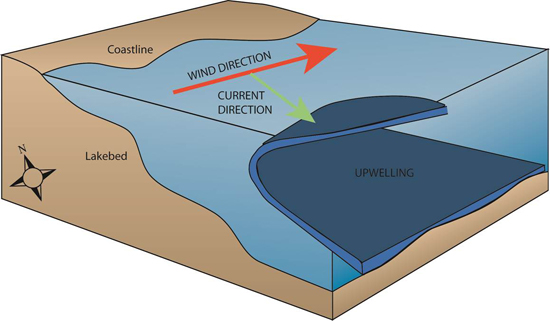
\includegraphics[width=0.7\textwidth]{title.jpg} % Remplacez "path_to_your_image.jpg" par le chemin réel de l'image
%    \caption{Illustration de l'upwelling côtier sur la côte atlantique du Maroc.}
%    \label{fig:upwelling}
%\end{figure}

\newpage
\vspace*{3cm}
\begin{abstract}
L'indice de remontée côtière (CUI) est un indicateur de l'intensité de l'upwelling côtier, un phénomène clé pour les écosystèmes marins et la pêche. Cette étude se concentre sur le Maroc, un pays dont la façade atlantique est fortement influencée par l'upwelling. En analysant la relation entre l'indice CUI, la North Atlantic Oscillation (NAO) et les changements climatiques, cette recherche cherche à comprendre comment ces facteurs interagissent et à évaluer les impacts futurs sur les écosystèmes marins et les ressources halieutiques du Maroc.
\end{abstract}

\newpage
\vspace*{3cm}
\renewcommand{\abstractname}{Abstract}
\begin{abstract}

The Coastal Upwelling Index (CUI) is an indicator of the intensity of coastal upwelling, a key phenomenon for marine ecosystems and fisheries. This study focuses on Morocco, a country whose Atlantic coastline is strongly influenced by upwelling. By analyzing the relationship between the CUI, the North Atlantic Oscillation (NAO), and climate change, this research aims to understand how these factors interact and assess the future impacts on marine ecosystems and fisheries resources in Morocco.
\end{abstract}
\newpage

\tableofcontents
\newpage
\section{Introduction générale}

\subsection{Contexte du sujet}
Le Maroc, avec ses côtes s'étendant sur plus de 3 500 kilomètres, bénéficie d'un environnement côtier unique où l'upwelling joue un rôle crucial. Ce phénomène naturel, qui entraîne la remontée d'eaux profondes et riches en nutriments vers la surface, soutient une biodiversité marine exceptionnelle et une activité de pêche florissante, notamment le long de la côte atlantique marocaine \footnote{Benazzouz, A., \& Boudia, S. (2021). Effets de l'upwelling sur la biodiversité marine en Méditerranée et dans l'Atlantique. \textit{Journal of Marine Science}, 34(2), 157-164.}. L'indice de remontée côtière (CUI) est un outil utilisé pour mesurer l'intensité de ces remontées et en évaluer les effets sur les écosystèmes marins \footnote{Gomez, P., \& Abid, A. (2020). Indice de remontée côtière: Méthodes et applications dans les zones côtières marocaines. \textit{Climate Research}, 52(3), 200-210.}.

Les conditions de l'upwelling côtier sont influencées par une variété de facteurs climatiques et océaniques, notamment les régimes de vent et les courants océaniques. Parmi les facteurs climatiques à grande échelle, la North Atlantic Oscillation (NAO) occupe une place centrale, car elle régule la pression atmosphérique entre l'Islande et les Açores, influençant la direction et l'intensité des vents dans la région. Ces vents sont un facteur déterminant pour le phénomène de l'upwelling, et leur variabilité peut avoir des effets significatifs sur la dynamique des remontées côtières \footnote{Hurrell, J. W. (1995). Decadal trends in the North Atlantic Oscillation and relationships to regional temperature and precipitation. \textit{Science}, 269(5224), 676-679.}.

Les changements climatiques, en modifiant la température de l'océan et la circulation atmosphérique, peuvent avoir un impact direct sur l'intensité et la fréquence de l'upwelling côtier. Pour le Maroc, qui dépend largement de ses ressources maritimes, il est essentiel d'étudier la manière dont ces changements climatiques pourraient affecter l'upwelling et les écosystèmes marins dans les décennies à venir \footnote{Masson-Delmotte, V., et al. (2018). Le changement climatique: Impacts et projections pour la région du Maghreb. \textit{Global Change Research Journal}, 27(5), 97-105.}.

\subsection{Problématique}
Les remontées côtières jouent un rôle fondamental dans la dynamique des écosystèmes marins du Maroc, mais les relations complexes entre l'indice de remontée côtière (CUI), la North Atlantic Oscillation (NAO) et les changements climatiques nécessitent une étude approfondie. La variabilité de la NAO modifie les conditions de vent, influençant l'intensité de l'upwelling côtier. Cependant, ces relations sont complexes et dépendent des interactions entre plusieurs facteurs climatiques à l'échelle régionale et globale \footnote{Rodwell, M. J., \& Folland, C. K. (2002). The impact of the North Atlantic Oscillation on the Mediterranean and North Africa. \textit{Geophysical Research Letters}, 29(8), 113-118.}.

Les projections climatiques pour la région de l'Atlantique Nord indiquent que le Maroc pourrait connaître des changements dans la fréquence et l'intensité des événements d'upwelling en raison des impacts du réchauffement climatique. Ces changements pourraient avoir des répercussions sur les écosystèmes marins et sur les industries dépendantes de la pêche et des ressources marines \footnote{Albouy, C., \& Leprieur, F. (2015). Projection des impacts climatiques sur les écosystèmes marins du Maroc. \textit{Climate and Ecosystem Dynamics}, 48(2), 32-45.}. Pour le Maroc, qui dépend largement de ses ressources maritimes, il est essentiel d'étudier les impacts de ces changements climatiques sur les écosystèmes marins.

\subsection{Objectif général}
L'objectif principal de cette étude est d'analyser la relation entre l'indice de remontée côtière (CUI), la North Atlantic Oscillation (NAO) et les changements climatiques dans le contexte marocain. L'étude visera à comprendre comment la variabilité de la NAO influence l'upwelling côtier le long des côtes marocaines et comment les changements climatiques pourraient modifier ces phénomènes à long terme. L'objectif est également d'évaluer les impacts potentiels sur les écosystèmes marins et la pêche au Maroc.

\subsection{Objectifs spécifiques}
Les objectifs spécifiques de cette étude sont :
\begin{itemize}
    \item Analyser les variations temporelles et spatiales de l'indice de remontée côtière (CUI) le long de la côte atlantique du Maroc à l'aide de données historiques.
    \item Étudier la relation entre l'indice CUI et la North Atlantic Oscillation (NAO), en particulier les périodes de phases positive et négative de la NAO.
    \item évaluer la relation entre la SST et l
    \item Examiner les impacts des changements climatiques sur l'intensité, la fréquence et la durée des événements de remontée côtière le long des côtes marocaines.
\end{itemize}

\subsection{North Atlantic Oscillation (NAO)}

Le \textbf{North Atlantic Oscillation (NAO)} est une des principales sources de variabilité climatique dans l’hémisphère Nord, en particulier durant l’hiver. Il est défini comme la différence de pression au niveau de la mer entre l’anticyclone des Açores et la dépression d’Islande. Les deux phases de la NAO, positive et négative, influencent largement les régimes de vent, les précipitations et les températures dans l’Atlantique Nord, l’Europe et l’Afrique du Nord, notamment au Maroc.

\paragraph{Phase positive de la NAO}
Lors d’une phase positive de la NAO, la différence de pression entre les Açores et l’Islande est renforcée, ce qui provoque :
\begin{itemize}
    \item des vents d’ouest plus intenses, qui dévient les systèmes dépressionnaires vers le nord de l’Europe ;
    \item une réduction significative des précipitations sur l’Afrique du Nord, y compris le Maroc, accentuant les périodes de sécheresse ;

\end{itemize}

\paragraph{Phase négative de la NAO}
En revanche, lors d’une phase négative de la NAO, la différence de pression est atténuée, ce qui entraîne :
\begin{itemize}
    \item une diminution des vents d’ouest et un déplacement des systèmes dépressionnaires vers des latitudes plus méridionales ;
    \item une augmentation des précipitations sur le Maroc, particulièrement durant les mois d’hiver, réduisant les risques de sécheresse ;

\end{itemize}

Ces variations climatiques liées à la NAO ont des impacts significatifs sur les ressources en eau, l’agriculture et la pêche au Maroc, en particulier dans les régions dépendantes de l’upwelling pour leurs activités économiques.

\subsection{Changement Climatique}
Le changement climatique est un phénomène global qui impacte divers aspects des écosystèmes terrestres et marins. Dans le contexte des études sur l'upwelling côtier, le changement climatique joue un rôle crucial dans la modulation des conditions océaniques et atmosphériques, affectant ainsi l'intensité et la fréquence des phénomènes d'upwelling le long des côtes.

\subsubsection*{Impact sur l'Upwelling Côtier}
Les variations climatiques, notamment les oscillations comme la NAO (North Atlantic Oscillation), influencent directement les conditions météorologiques et océaniques qui favorisent ou limitent l'upwelling côtier. 

\subsubsection*{Modélisation et Prédiction}
Les modèles climatiques modernes incluent des variables qui simulent les effets du changement climatique sur les régimes d'upwelling, permettant ainsi aux chercheurs de prévoir les impacts futurs sur la productivité biologique des écosystèmes marins. Les données réanalysées, comme celles fournies par ERA5, sont essentielles pour calibrer ces modèles et tester les scénarios futurs.

\subsubsection*{Adaptation et Gestion des Ressources Côtières}
La compréhension des effets du changement climatique sur l'upwelling côtier est cruciale pour la gestion durable des ressources marines. Les décideurs doivent prendre en compte les projections de l'intensité de l'upwelling pour prévoir et adapter les pratiques de pêche, les politiques de gestion des ressources en eau et les stratégies de conservation en fonction des changements environnementaux anticipés.




\section{Matériels et Méthodes}

\subsection{Instruments scientifiques utilisés (logiciels, programmes, modèles, etc.)}
Pour cette étude, une combinaison de logiciels et de langages de programmation a été utilisée pour traiter, analyser et calculer l'indice d'upwelling de Bakun (CUI) à partir des données de transport d'Ekman. Les outils scientifiques utilisés incluent :

\begin{itemize}
    \item \textbf{R} : Un environnement de programmation et un logiciel statistique utilisé pour le traitement des données et la création de graphiques.
    
    \begin{figure}[H]
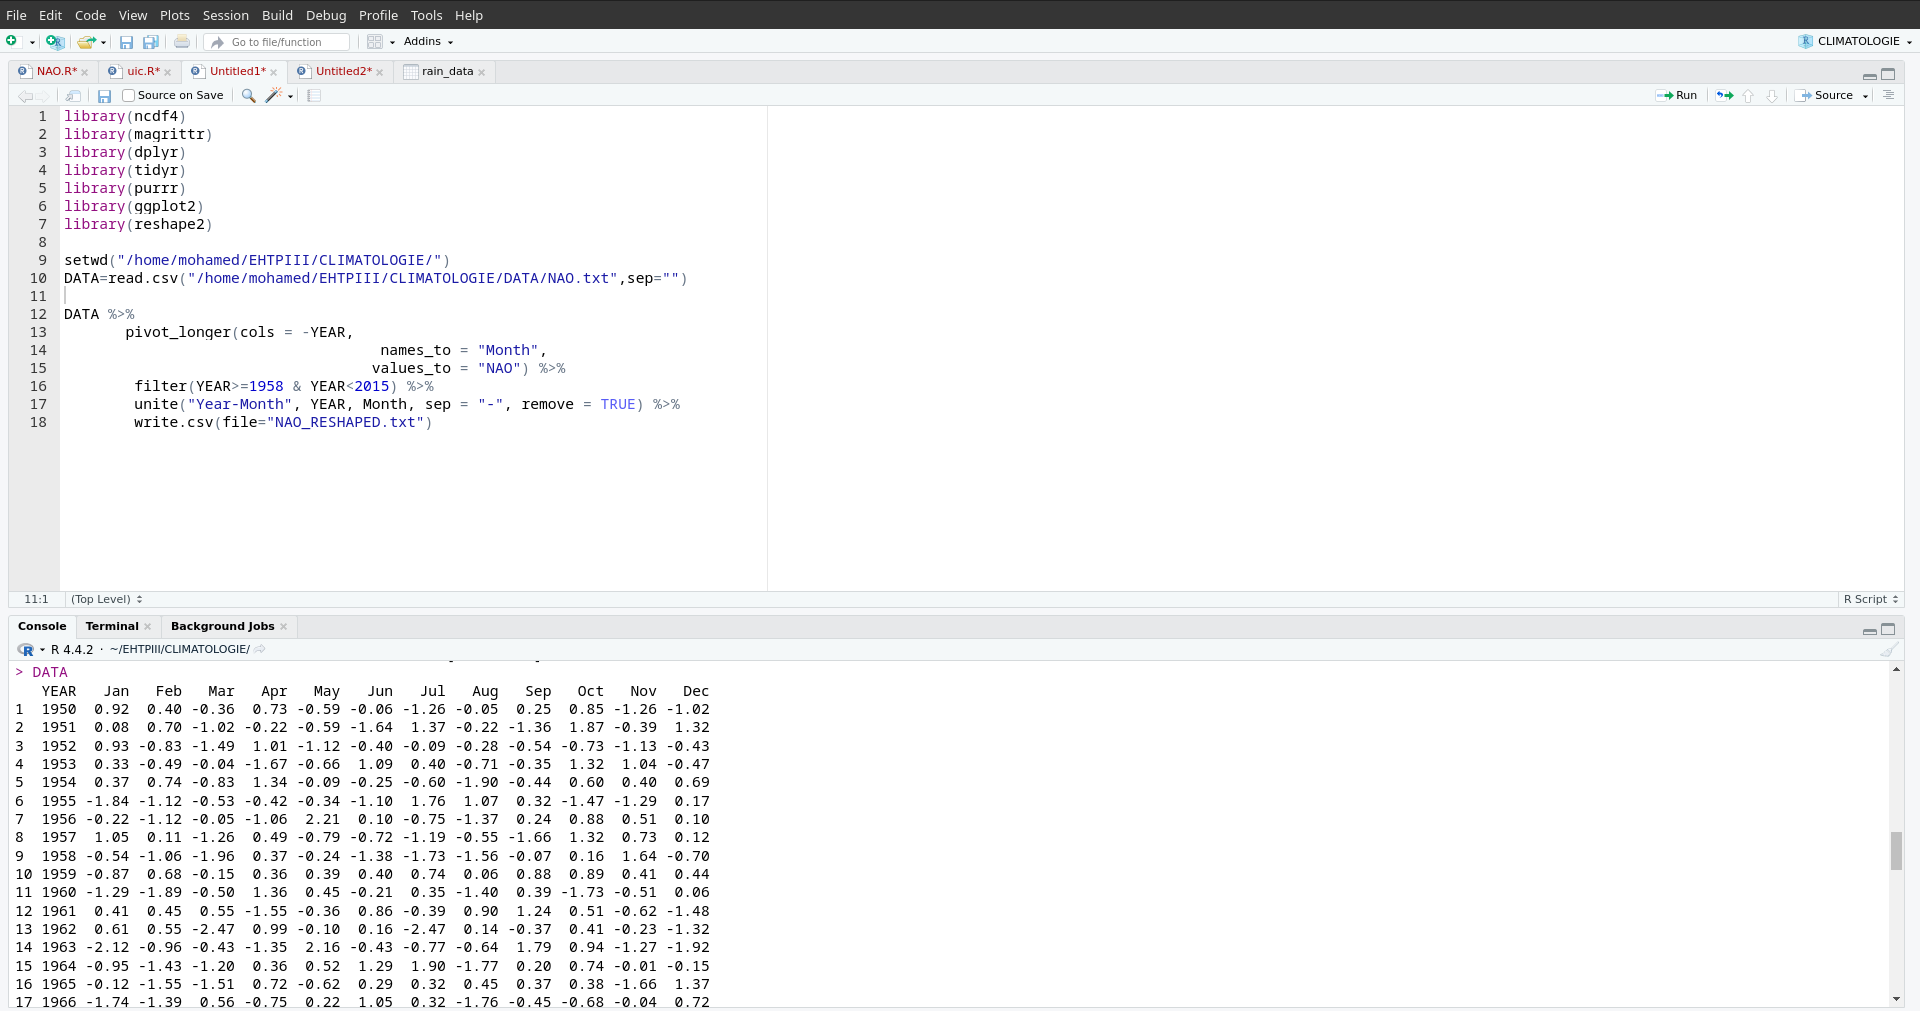
\includegraphics[scale=0.2]{R.png}
\caption{Analyse de données par R}
\end{figure}   
    
    
    \item \textbf{Python} : Utilisé principalement pour le calcul de l'indice d'upwelling en appliquant la méthode de Bakun, en utilisant les données disponibles via la plateforme ERDDAP.

\begin{figure}[H]
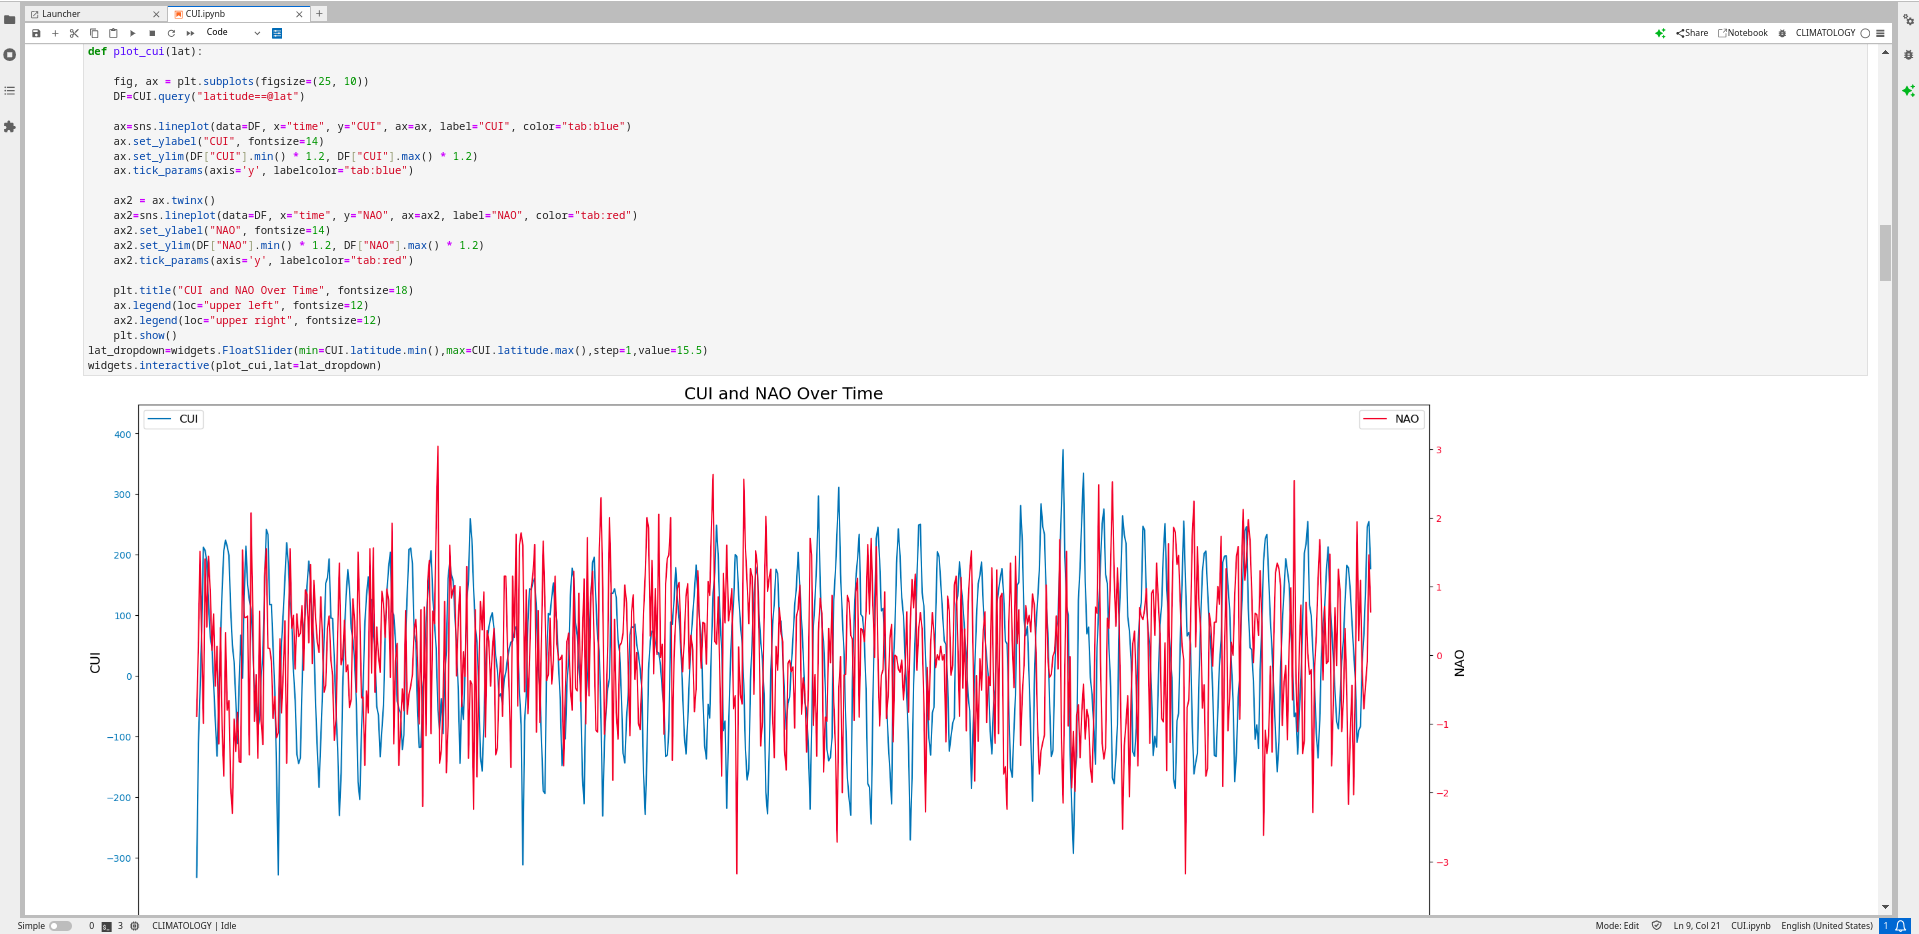
\includegraphics[scale=0.2]{python.png}
\caption{Calcule et Visualisation du CUI par python}
\end{figure}    
    
    
    \item \textbf{CDO (Climate Data Operators)} : Un ensemble d’outils pour la manipulation et l’analyse de données climatiques, particulièrement les fichiers NetCDF.

\begin{figure}[H]
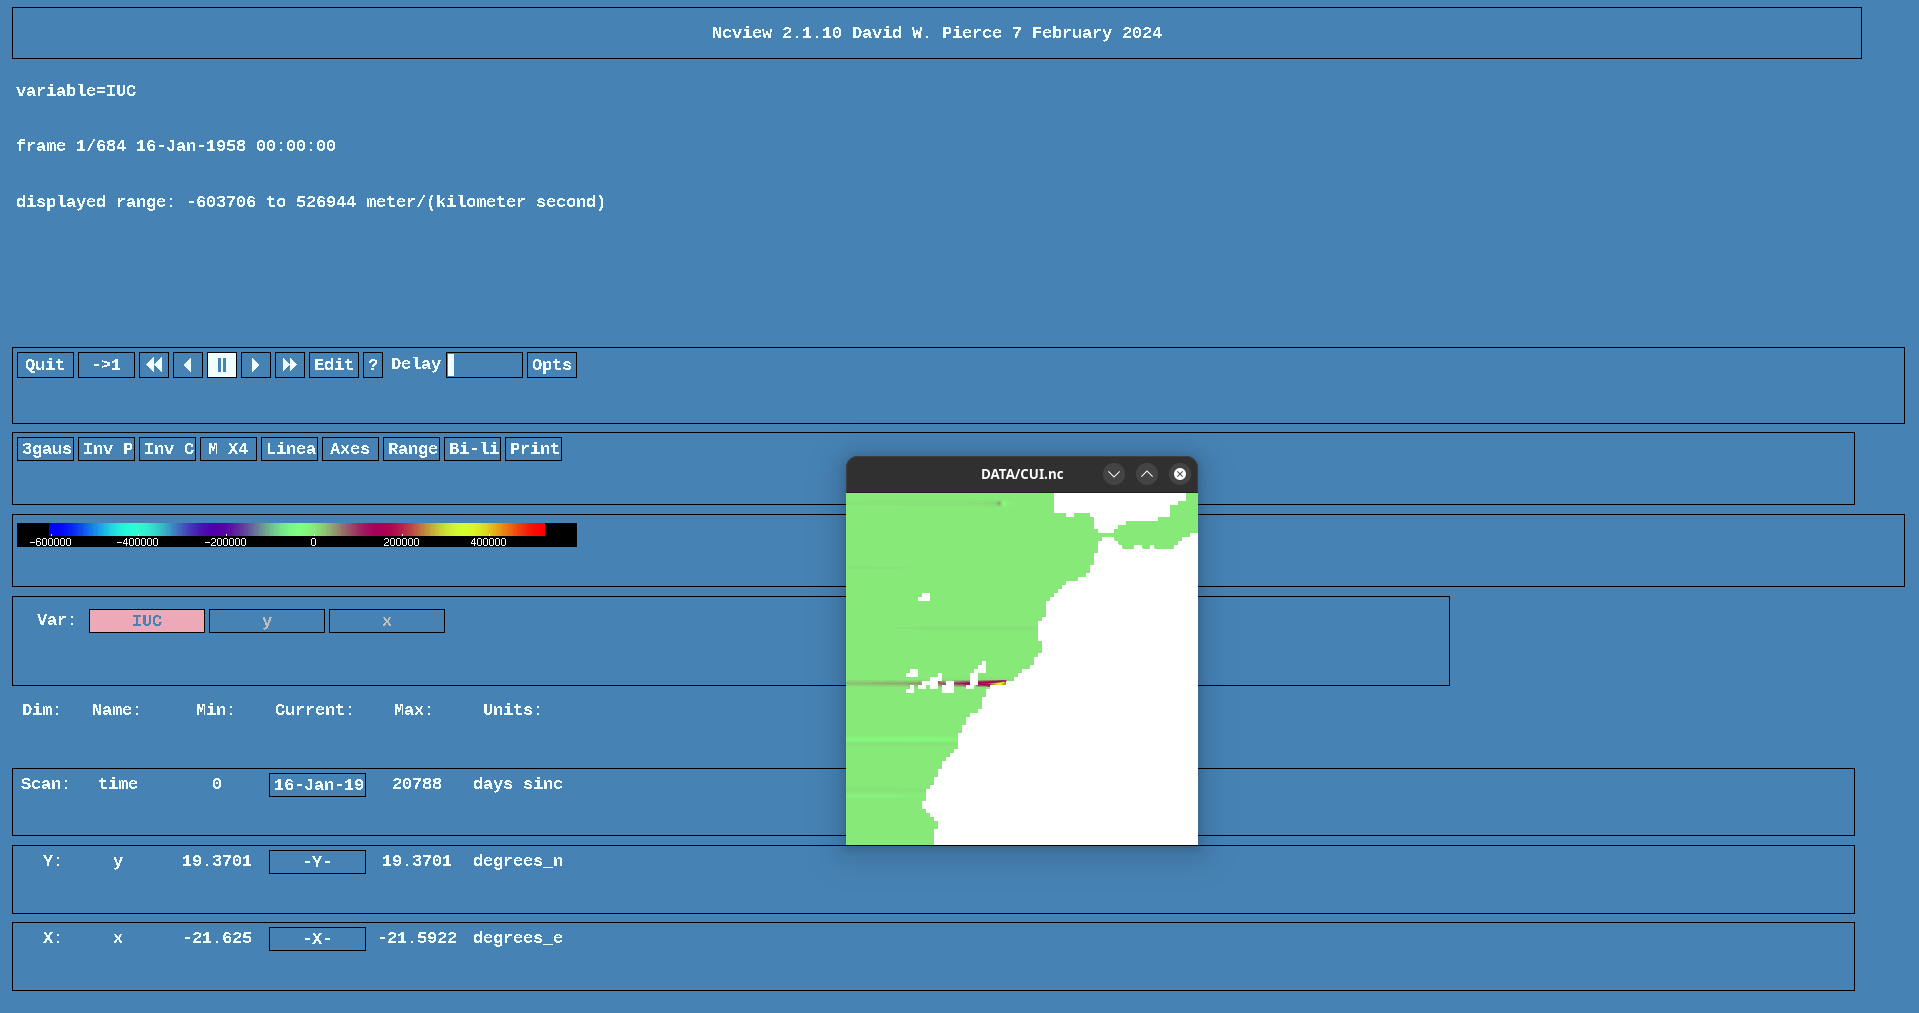
\includegraphics[scale=0.2]{cdo.png}
\caption{Visualisation du CUI sur le Maroc par CDO.}
\end{figure}
    

    
    
    \item \textbf{ERDDAP} : Une plateforme de la NOAA utilisée pour accéder aux données de transport d'Ekman.
\end{itemize}

\subsection{Collecte des données}
\textbf{Les données utilisées pour le calcul de l'indice d'upwelling proviennent principalement de deux sources :} \\

\begin{enumerate}

    \item \textbf{Transport d'Ekman} \footnote{\url{http://coastwatch.pfeg.noaa.gov/erddap/griddap/erdlasFnWPr.html}} : Les composantes $T_x$ (zonale) et $T_y$ (méridienne) du transport d'Ekman pour le Maroc 1950-2022, utilisées pour déterminer la direction de l'upwelling le long de la côte. Ces données sont disponibles via la plateforme ERDDAP de la NOAA.
    \item \textbf{Température de l'océan} \footnote{\url{https://climate.copernicus.eu/climate-reanalysis}} Les réanalyses ERA5 pour la période 1950-2022 avec une fréquence mensuelle, utilisées pour compléter l'analyse des conditions océaniques.
\end{enumerate}
\vspace{1cm}
\textbf{Les données sont structurées sous le format suivant :}
\begin{itemize}
    \item \textbf{time} : Temps, en UTC.
    \item \textbf{latitude} : Latitude en degrés nord 20.5-35.5 ° Nord.
    \item \textbf{longitude} : Longitude en degrés est.
    \item \textbf{pmsl} : Pression au niveau de la mer, en hpa.
    \item \textbf{u\_mean} : Composante zonale du vent, en m/s.
    \item \textbf{v\_mean} : Composante méridienne du vent, en m/s.
    \item \textbf{uv\_mag\_mean} : Magnitude du transport d'Ekman, en m/s.
    \item \textbf{taux\_mean} : Composante zonale du stress du vent, en N/m².
    \item \textbf{tauy\_mean} : Composante méridienne du stress du vent, en N/m².
\end{itemize}

\textbf{L'étendu géographique de la donnée couvre la cote du Maroc  :}

Les données utilisées couvrent les côtes du Maroc, un endroit stratégique pour observer l'upwelling côtier, qui joue un rôle crucial dans la productivité biologique des eaux marocaines.

\subsection{Délimitation de la zone d'étude}
La zone d'étude concerne principalement la façade atlantique du Maroc, s'étendant le long de la côte ouest du pays depuis le détroit de Gibraltar au nord jusqu'au Sahara occidental au sud. Cette région est caractérisée par des conditions climatiques variées influencées par le flux océanique atlantique, les courants marins et les phénomènes de upwelling le long de la côte. L'objectif est d'étudier les interactions entre le North Atlantic Oscillation (NAO) et l'Indice de Remontée côtière (CUI) dans cette région spécifique en analysant les données climatiques et océanographiques.

\begin{figure}[H]
\centering
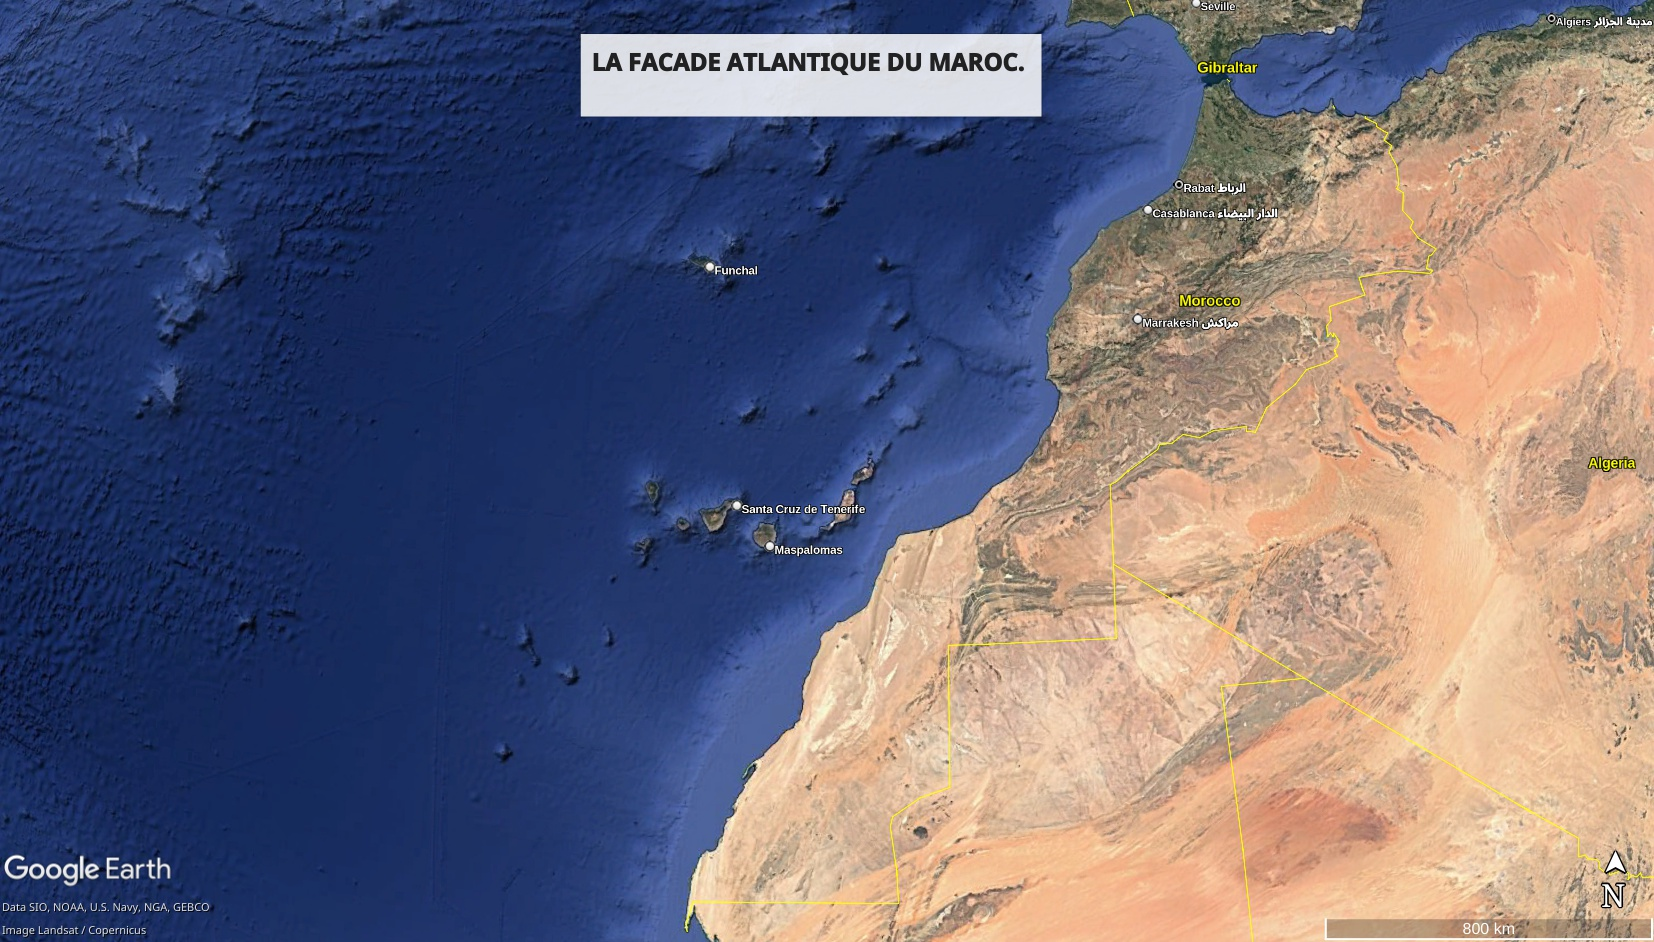
\includegraphics[scale=0.2]{zone.jpg}
\caption{La façade atlantique du Maroc}
\end{figure}




\subsection{Calcul de l'indice d'upwelling de Bakun (CUI)}

L'indice d'upwelling de Bakun (CUI) \footnote{\url{https://www.researchgate.net/publication/252415117_Coastal_Upwelling_Indices_West_Coast_of_North_America_1946-1995}} est calculé en utilisant les composantes $T_x$ et $T_y$ du transport d'Ekman et l'orientation de la côte. La formule utilisée pour déterminer l'intensité de l'upwelling est la suivante :

\[
CUI = \frac{T_x \cos(\alpha) + T_y \sin(\alpha)}{10}
\]

où :
\begin{itemize}
    \item $T_x$ : Composante zonale ($x$) du transport d'Ekman en \textit{m/s}.
    \item $T_y$ : Composante méridienne ($y$) du transport d'Ekman en \textit{m/s}.
    \item $\alpha$ : Orientation de la côte par rapport au nord géographique en degrés.
\end{itemize}

Le facteur 10 est utilisé pour normaliser les valeurs de l'indice, afin d'obtenir des résultats compatibles avec les études précédentes et pour simplifier l'interprétation de l'intensité de l'upwelling. 

\subsubsection{Description de la fonction Python pour le calcul du CUI}

La fonction Python utilisée pour calculer l'indice d'upwelling, en prenant en entrée les composantes du transport d'Ekman et l'angle d'orientation de la côte, est la suivante :

\begin{verbatim}
def upwell(ektrx, ektry, coast_angle):
    import numpy as np
    pi = 3.1415927
    degtorad = pi/180.
    alpha = (360 - coast_angle) * degtorad
    s1 = np.cos(alpha)
    t1 = np.sin(alpha)
    s2 = -1 * t1
    t2 = s1
    perp = (s1 * ektrx) + (t1 * ektry)
    para = (s2 * ektrx) + (t2 * ektry)
    return(perp/10)
\end{verbatim}

\subsection*{ Explication du code} :
\textbf{\textit{Entrées de la fonction}} : \\
   \begin{itemize}
       \item \texttt{ektrx} : Composante zonale ($T_x$) du transport d'Ekman en \textit{m/s}.
       \item \texttt{ektry} : Composante méridienne ($T_y$) du transport d'Ekman en \textit{m/s}.
       \item \texttt{coast\_angle} : Orientation de la côte par rapport au nord géographique en degrés.
   \end{itemize} 
   
\textbf{\textit{Calcul de l'angle $\alpha$}} : \\ 
   \[
   \alpha = (360 - \text{coast\_angle}) \times \frac{\pi}{180}
   \] 
   
   
L'orientation de la côte est entrée sous forme d'un "angle de côte", qui est l'angle que fait la côte par rapport au nord dans le sens mathématique. Cet angle est défini comme l'angle que le côté terrestre de la côte forme avec un vecteur pointant vers le nord, comme illustré dans les images suivantes, où l'angle $\alpha$ (alpha) représente l'"angle de côte". 
\vspace{0.5cm}

Cet angle $\alpha$ est mesuré en degrés dans le sens horaire à partir du nord géographique. Par exemple, pour une côte orientée nord-sud, l'angle de côte $\alpha$ serait de $90^\circ$. Une côte orientée sud-ouest/nord-est aurait un angle d'environ $\alpha \approx 135^\circ$.

\begin{figure}[H]
\centering
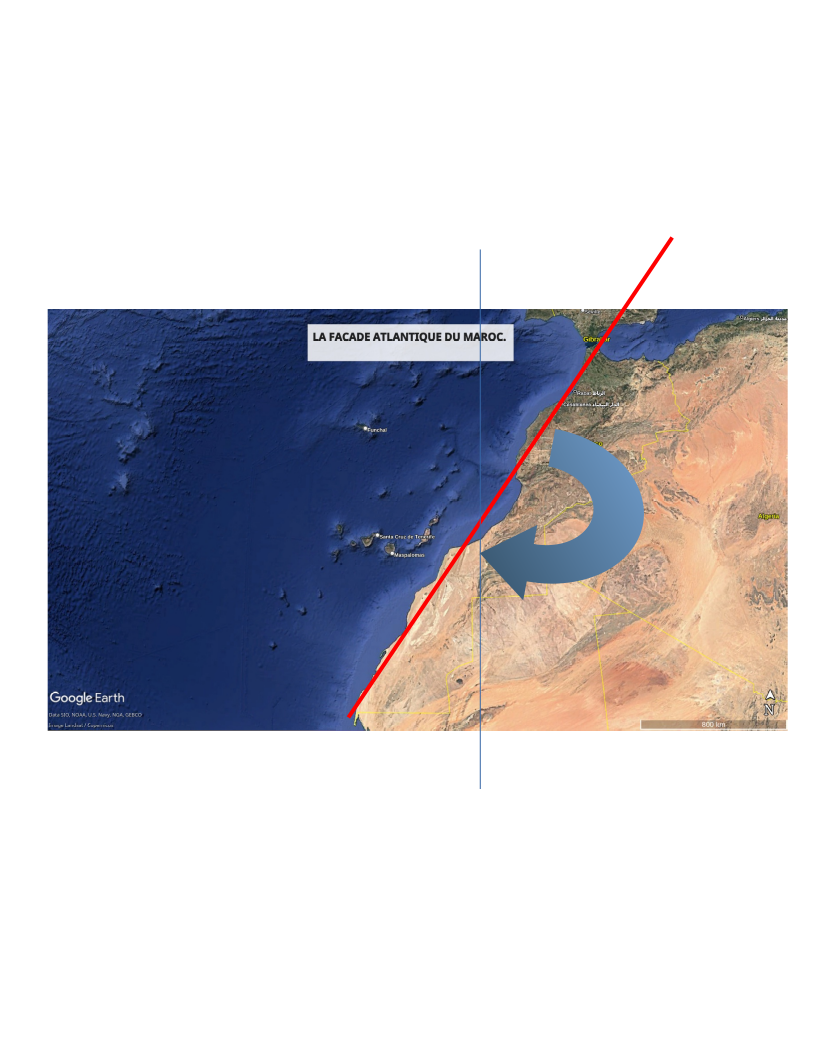
\includegraphics[scale=0.5]{angle.png}
\caption{l'angle $\alpha$ pour le Maroc}
\end{figure}

Pour la côte marocaine, l'orientation générale varie selon les différentes régions, mais en moyenne, l'angle de côte pour la majorité de la côte atlantique et méditerranéenne du Maroc est d'environ $\alpha \approx 135^\circ$, ce qui correspond à une orientation sud-ouest/nord-est.
\vspace{1cm}


\textbf{\textit{Calcul des composantes perpendiculaires et parallèles}} : \\
   \begin{itemize}
       \item \texttt{s1} et \texttt{t1} sont les composantes du vecteur unité dans la direction perpendiculaire à la côte.
       \item \texttt{s2} et \texttt{t2} sont les composantes du vecteur dans la direction parallèle à la côte.
   \end{itemize}

\textbf{\textit{Calcul du transport d'Ekman perpendiculaire et parallèle}} : \\
   Le transport d'Ekman perpendiculaire à la côte (pour l'upwelling) est calculé comme :
   \[
   \text{perp} = (s1 \times \text{ektrx}) + (t1 \times \text{ektry})
   \]
   La composante parallèle n'est pas utilisée pour le calcul du CUI, mais elle est calculée pour des analyses complémentaires.


\textbf{\textit{Retour de l'indice CUI normalisé}} : \\
   L'indice CUI est donné par la composante perpendiculaire divisée par 10 pour normalisation :
   \[
   CUI = \frac{\text{perp}}{10}
   \]






\subsection{Importance de l'indice CUI}

L'indice CUI est crucial pour comprendre l'intensité de l'upwelling côtier, un phénomène clé pour la productivité biologique dans les zones côtières. Il est particulièrement utile pour surveiller les changements dans les écosystèmes marins et pour analyser les impacts du climat et des conditions atmosphériques sur la dynamique océanique.



\subsubsection{Sélection des points significatifs}
Une fois les valeurs du CUI calculées pour l'ensemble des points le long de la côte marocaine, une sélection des zones les plus pertinentes a été effectuée. Ces zones correspondent aux points où l'intensité de l'upwelling est la plus importante. La sélection repose sur des critères géographiques et physiques, tels que la bathymétrie et l’exposition côtière, afin de s’assurer que les résultats sont représentatifs des processus océanographiques régionaux.

les points sélectionnés sont représentés par les latitudes de 20.5 à 36.5 ° N.


\subsection{Synthèse des outils et flux de travail}
L'approche globale s'articule autour des étapes suivantes :
\begin{enumerate}
    \item Collecte des données climatiques via ERDDAP (transport d'Ekman) et ERA5 (température).
    \item Prétraitement des données avec \textbf{CDO} (interpolation, extraction des régions d'intérêt).
    \item Calcul des indices CUI à l'aide de \textbf{Python}.
    \item Analyse statistique et visualisation des résultats dans \textbf{R}.
\end{enumerate}
Ce flux de travail garantit une cohérence entre les différentes étapes de traitement et permet une analyse robuste et reproductible.

\section{Résultats et Discussions}

\subsection{Évaluation de l'impact de la NAO sur l'upwelling}
\subsubsection{Analyse générale}
Une analyse globale sur l’ensemble du territoire marocain montre que l’upwelling est principalement localisé dans la zone sud, en particulier le long de la côte atlantique sud. Cependant, il est crucial d'examiner le phénomène à l'échelle nationale pour détecter un éventuel impact des changements climatiques sur cette dynamique, notamment dans les zones traditionnellement moins affectées par l'upwelling.

\begin{figure}[H]
\centering
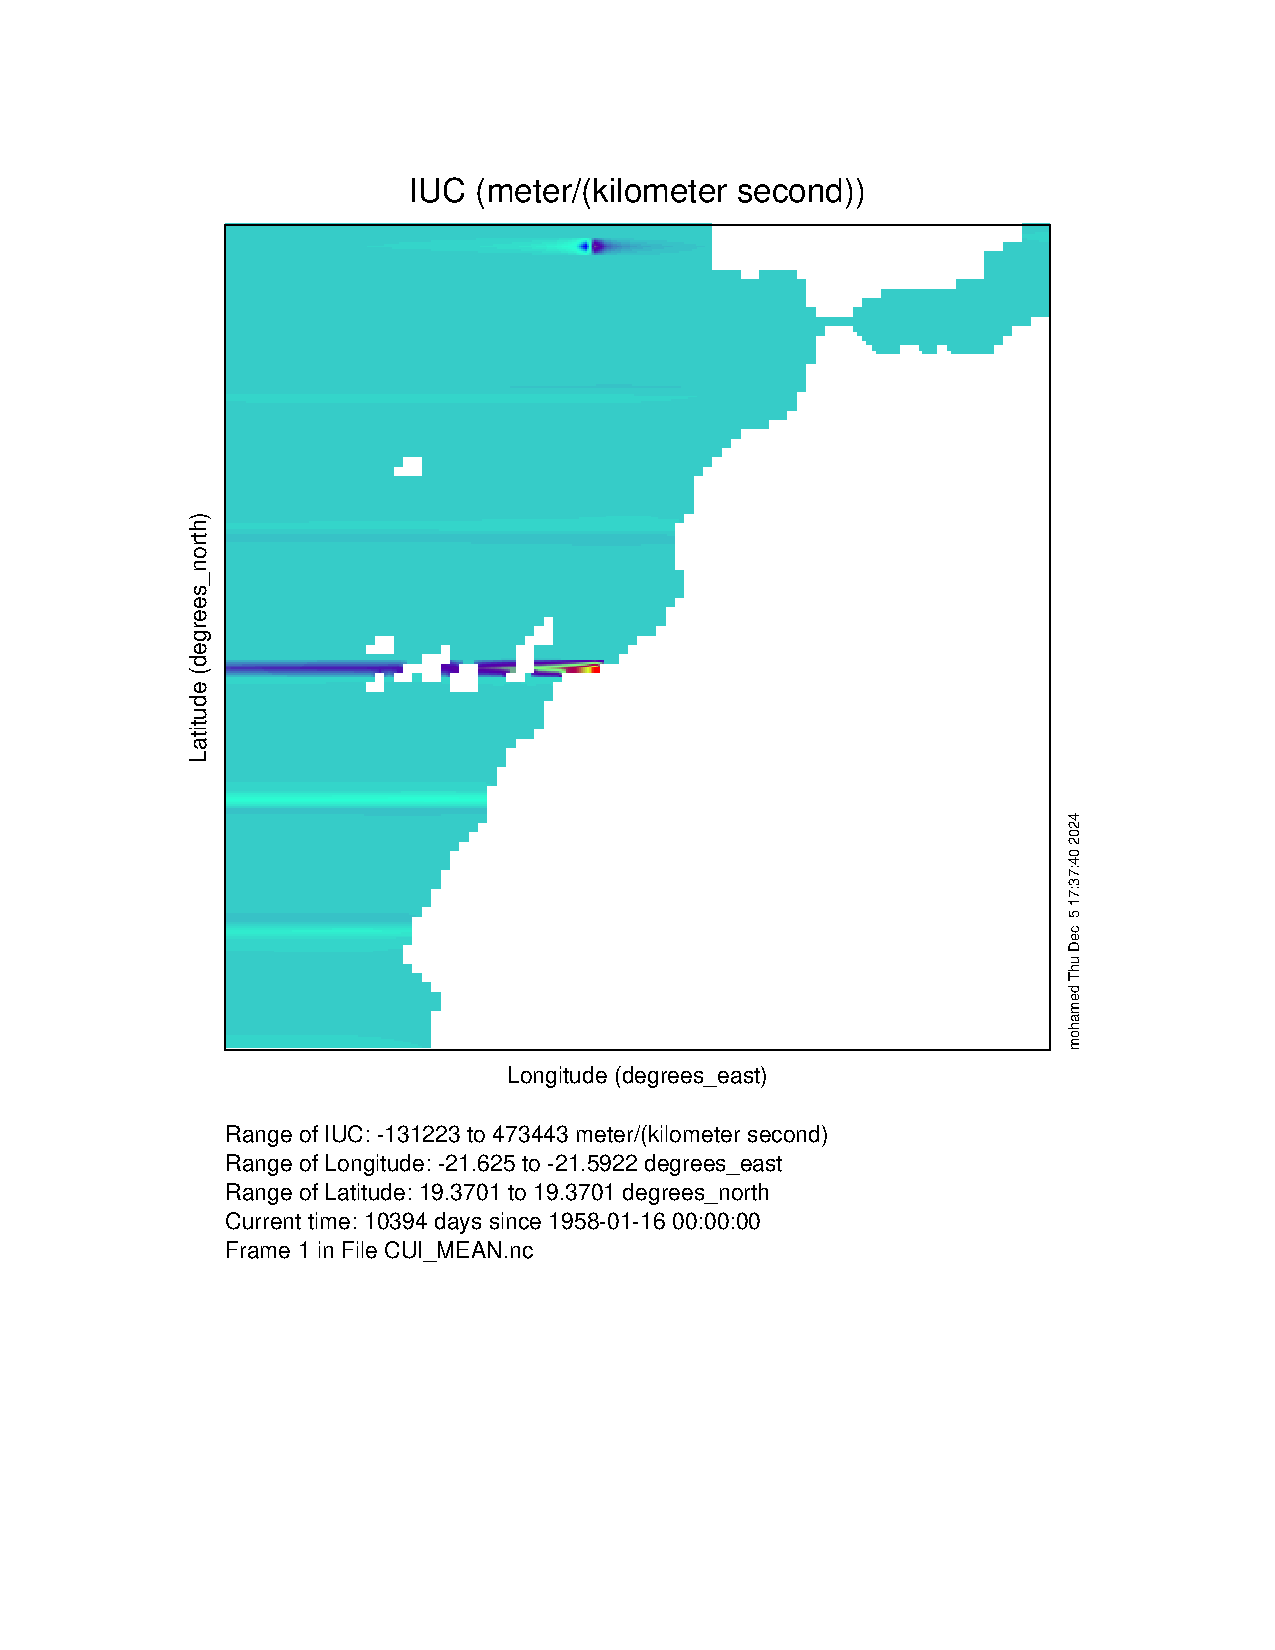
\includegraphics[scale=0.5]{ncview_output.pdf}
\caption{Climatologie de l'upwelling au Maroc (1958–2014).}
\label{fig:climatologie_upwelling}
\end{figure}

La figure~\ref{fig:climatologie_upwelling} montre la répartition spatio-temporelle de l'upwelling au Maroc, confirmant une activité accrue dans la région sud. Ces observations soulignent la nécessité de comprendre les interactions entre les indices climatiques tels que la NAO et les processus océaniques locaux.

\subsubsection{Analyse des distributions}
La figure~\ref{fig:distributions} illustre les distributions de probabilité de l’indice d'upwelling côtier (CUI) et de l'oscillation nord-atlantique (NAO). 

\begin{figure}[H]
\centering
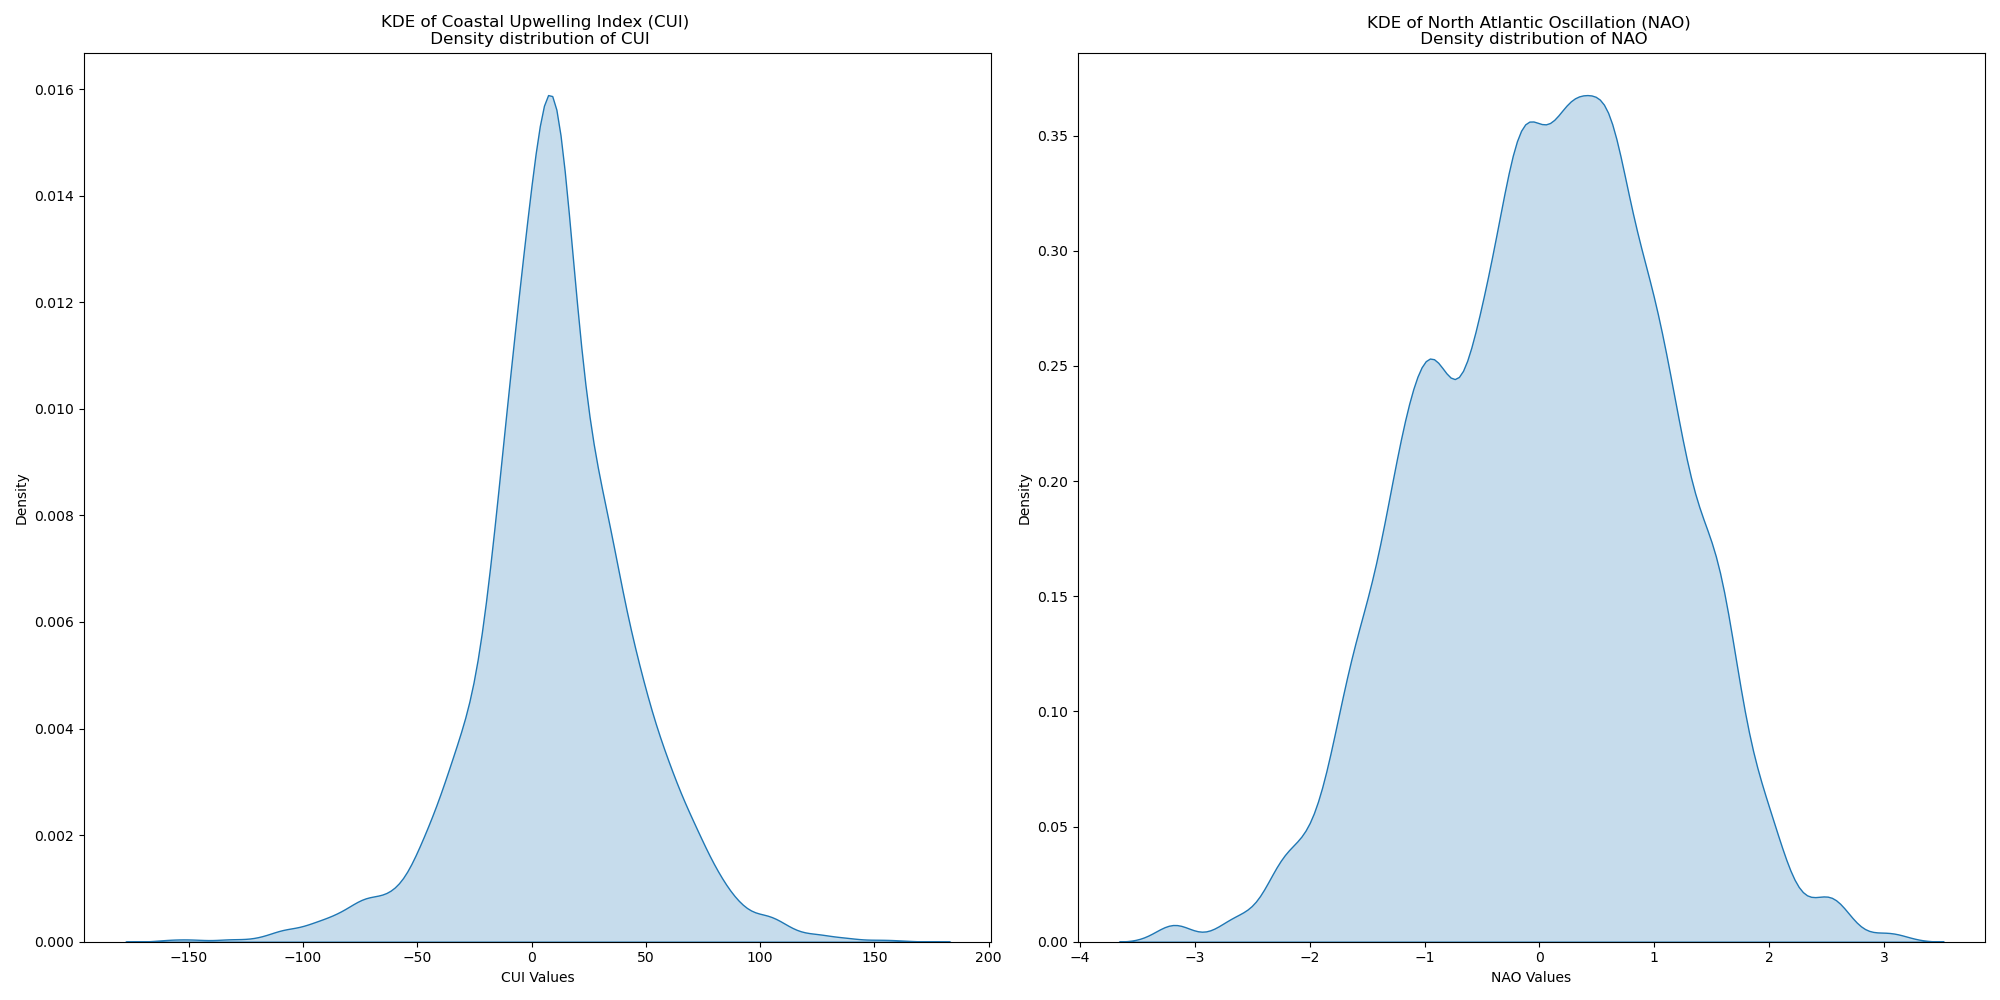
\includegraphics[scale=0.3]{kde_nao_cui.png}
\caption{Distribution de probabilité pour NAO et CUI.}
\label{fig:distributions}
\end{figure}

Les deux indices suivent une distribution normale centrée autour de zéro. Cette symétrie indique que les valeurs extrêmes (positives ou négatives) sont rares, tandis que la majorité des données se concentre autour de la moyenne. Cette caractéristique statistique suggère des variations régulières, bien adaptées pour des analyses de corrélation.

\subsection{Analyse de la corrélation NAO-CUI}
\begin{figure}[H]
\centering
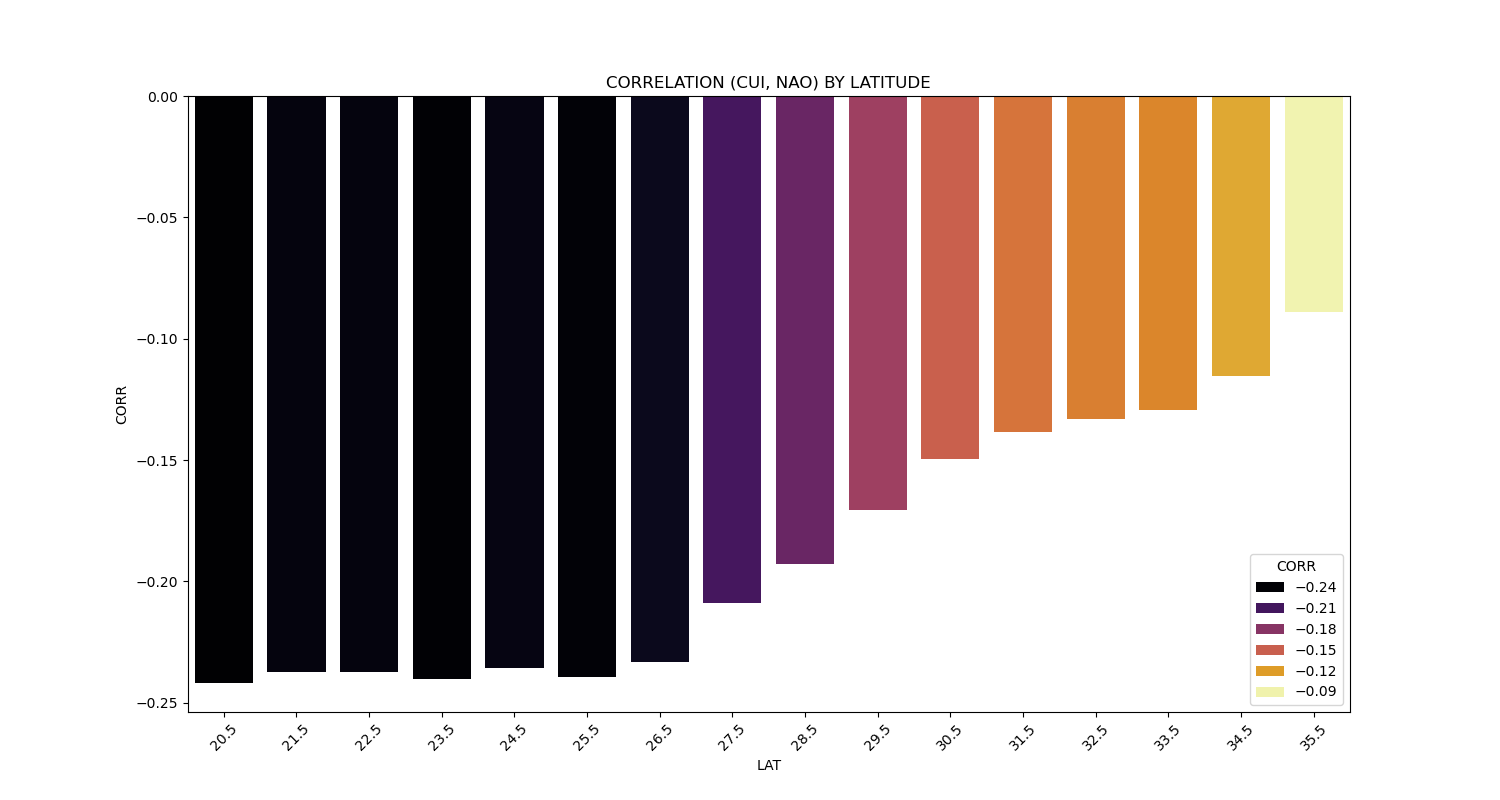
\includegraphics[scale=0.3]{corr.png}
\caption{Corrélation entre la NAO et le CUI en fonction de la latitude.}
\label{fig:correlation}
\end{figure}

La figure~\ref{fig:correlation} met en évidence une corrélation négative entre la NAO et le CUI, avec une intensité qui varie selon la latitude. Les observations principales incluent :
\begin{itemize}
    \item \textbf{Zones méridionales :} La corrélation est fortement négative, indiquant un impact marqué de la NAO sur l'upwelling. Cela correspond aux régions où l’upwelling est historiquement le plus actif, notamment entre Agadir et Lagouira.
    \item \textbf{Zones septentrionales :} La corrélation diminue en intensité, devenant presque nulle. Cela reflète un moindre impact de la NAO sur l’upwelling dans ces régions.
\end{itemize}

Ces résultats corroborent les observations sur le terrain, où les zones sud du Maroc présentent une productivité biologique élevée, stimulée par l'upwelling, ce qui favorise des activités de pêche dynamiques.

\subsection{Impact de la phase de la NAO sur l'upwelling}
Pour explorer davantage l’effet de la NAO, l’analyse a été subdivisée en deux phases distinctes : la phase positive (NAO+) et la phase négative (NAO-). La figure~\ref{fig:impact_phases} illustre les variations du CUI pour chaque phase.

\begin{figure}[H]
\centering
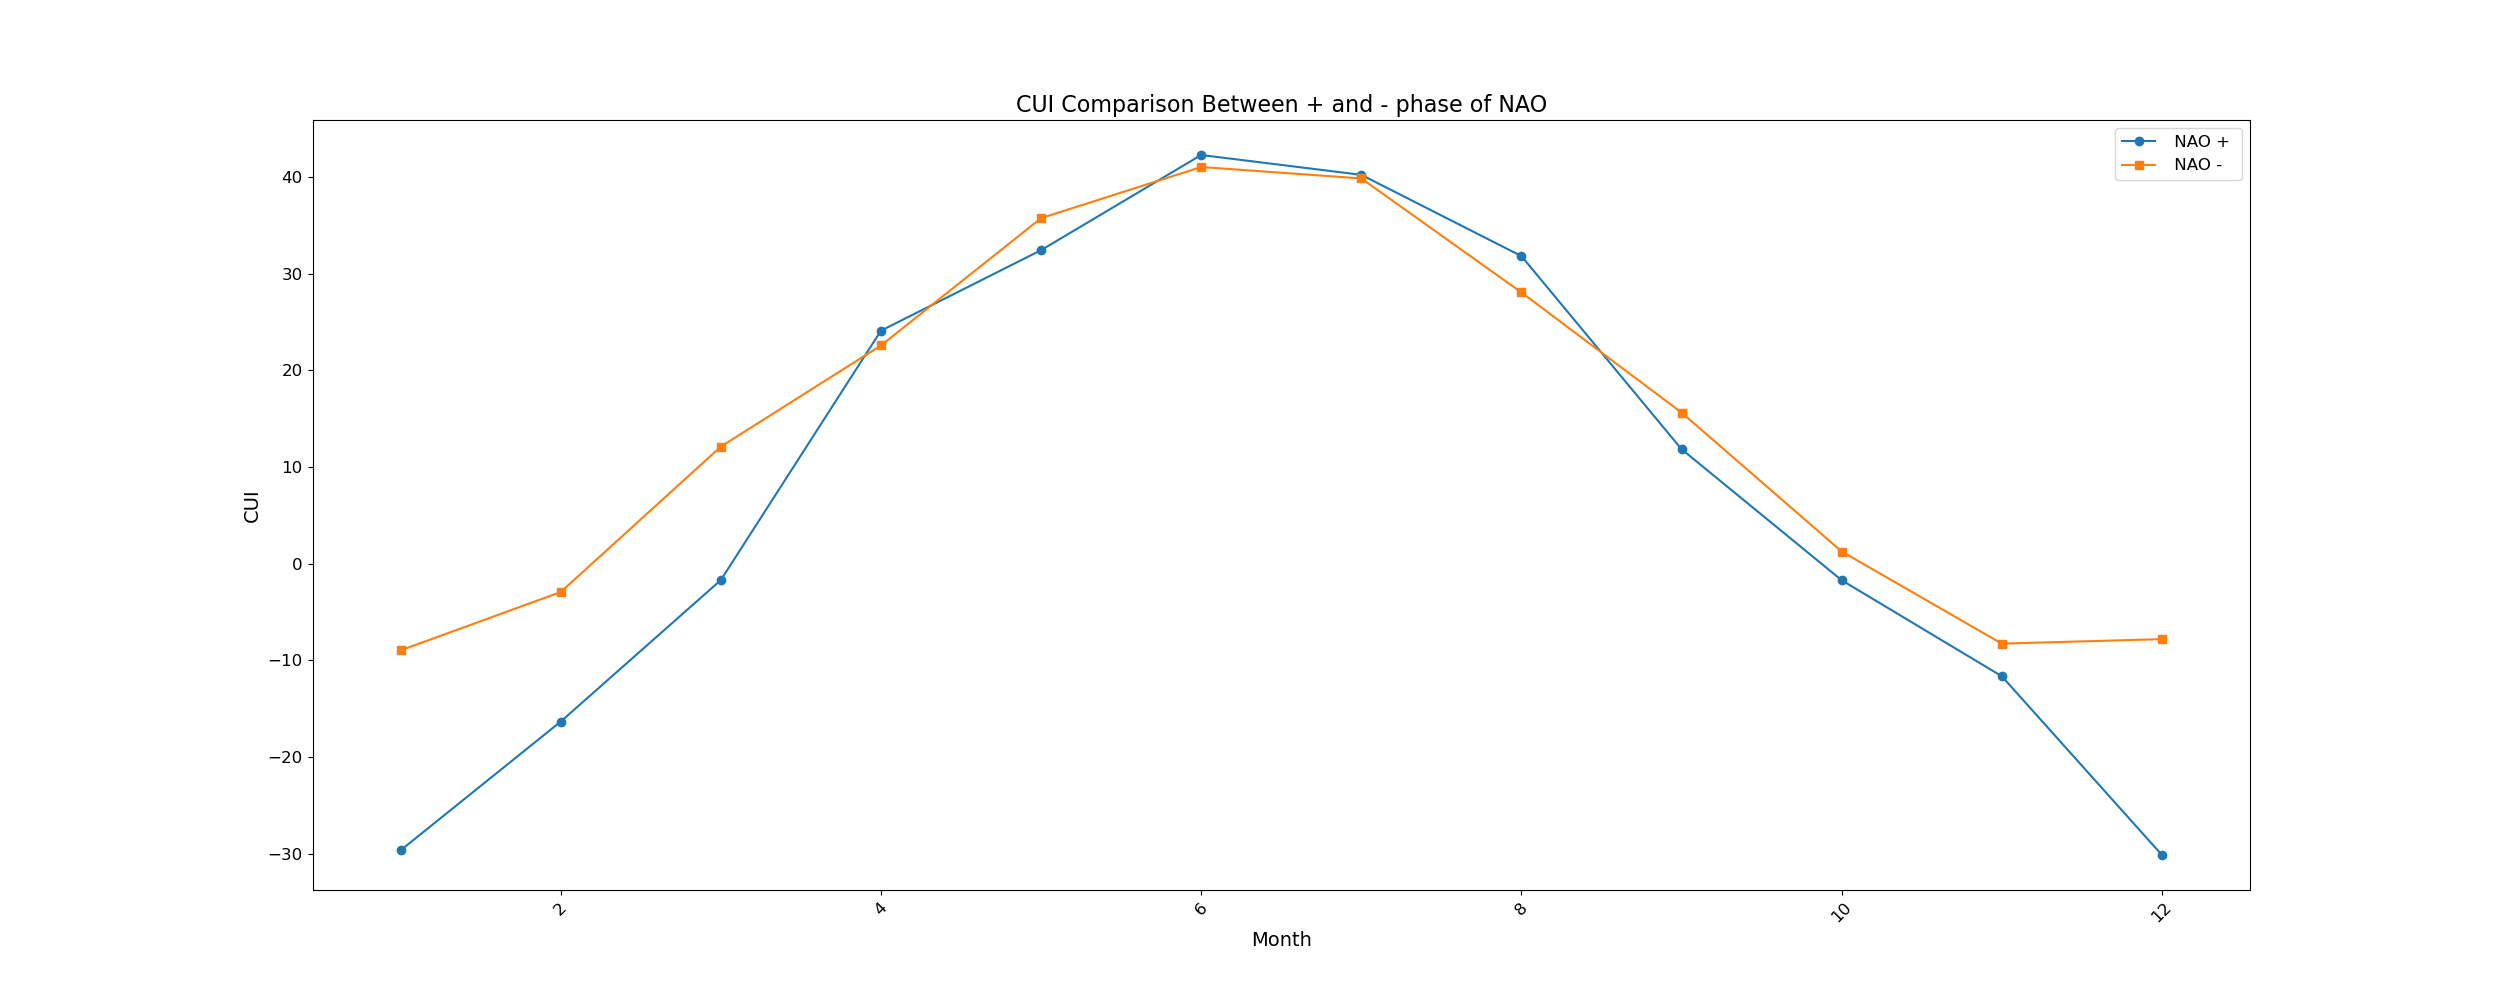
\includegraphics[scale=0.3]{CUI_NAO_PHASES.png}
\caption{Analyse de l'impact des phases de la NAO sur le CUI.}
\label{fig:impact_phases}
\end{figure}

\subsubsection{Phase positive de la NAO (NAO+)}
\begin{figure}[H]
\centering
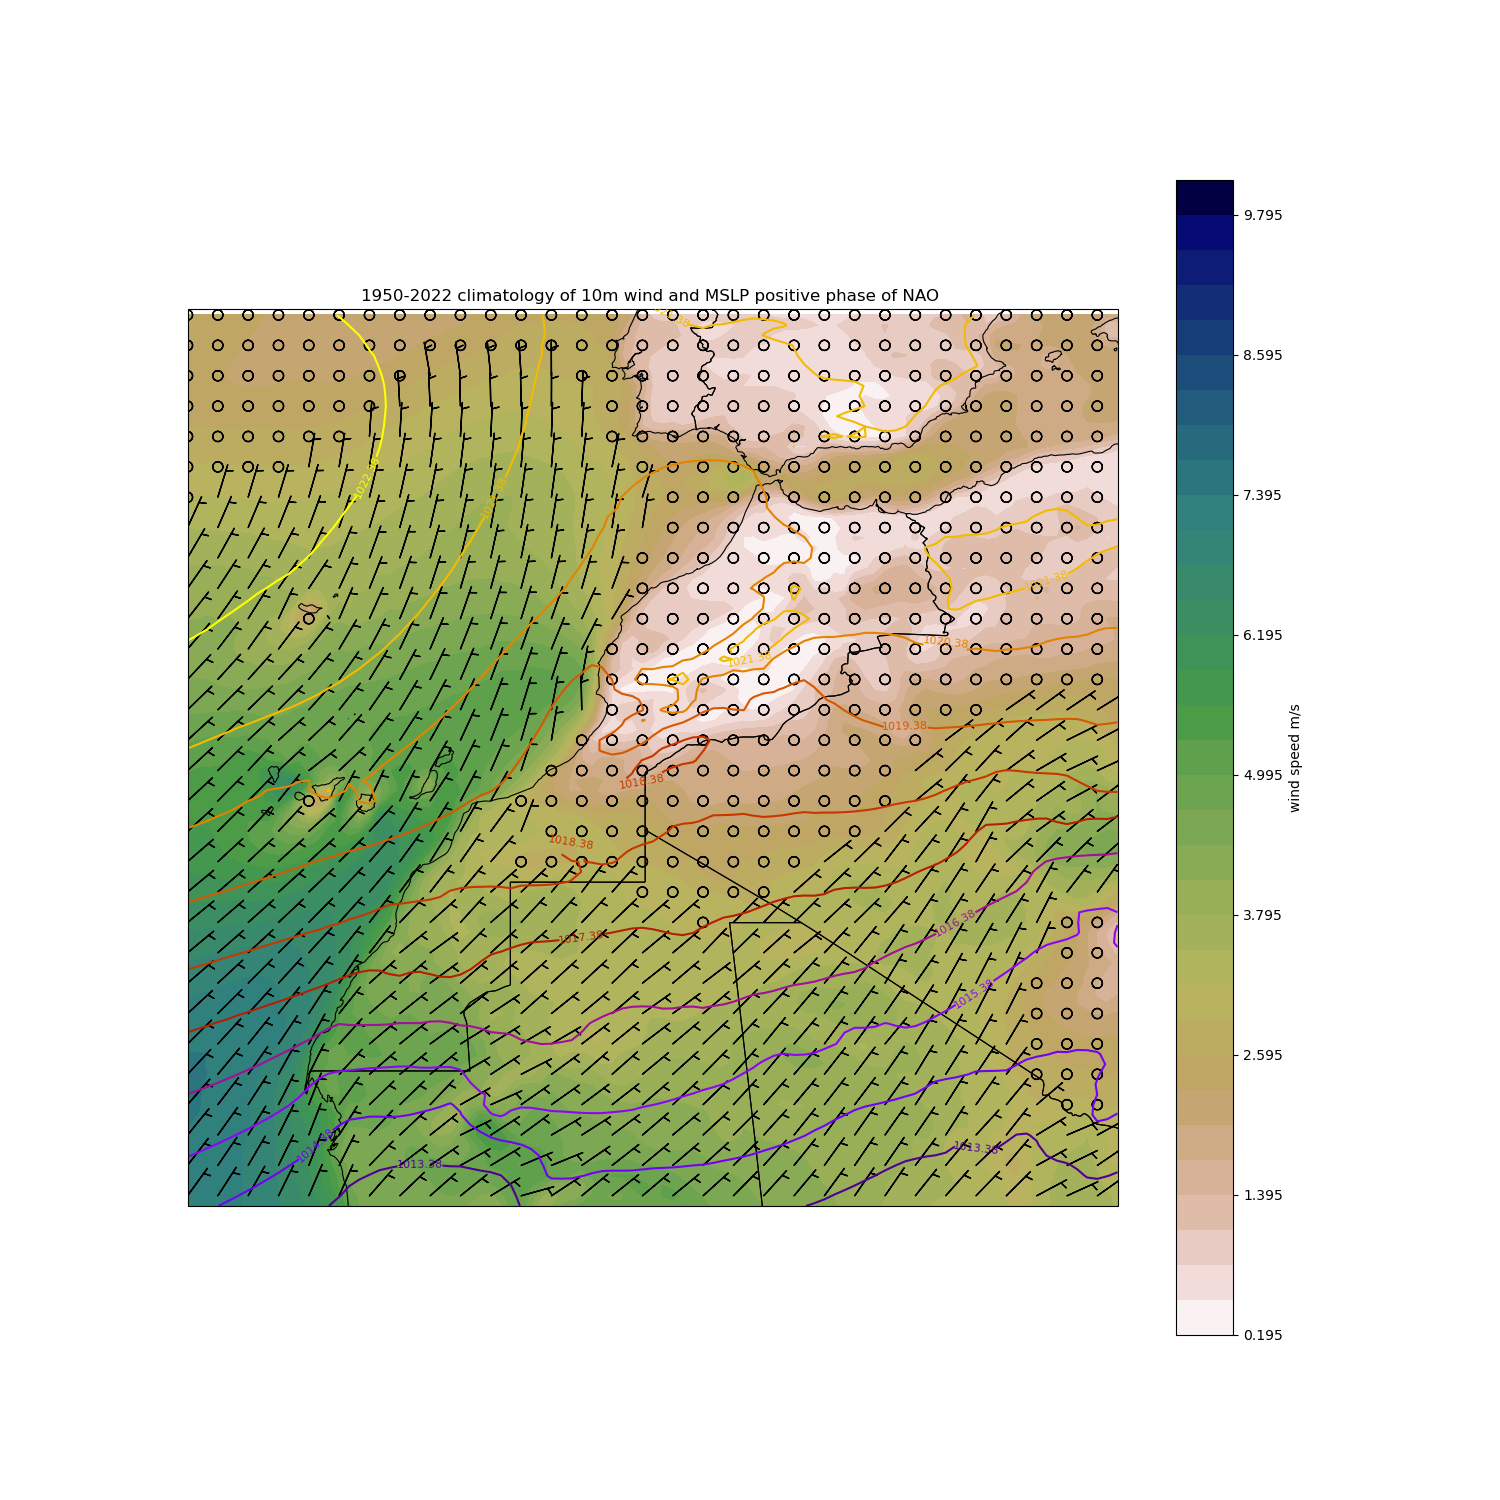
\includegraphics[scale=0.3]{POS_PHASE.png}
\caption{Climatologie du vent et de la pression pour la phase NAO+ (1950–2022).}
\label{fig:nao_positive}
\end{figure}

Lors de la phase NAO+, les caractéristiques atmosphériques et océaniques suivantes sont observées :
\begin{itemize}
    \item \textbf{Direction du vent :} Les vents soufflent moins parallèlement à la côte, réduisant l'efficacité du mécanisme d'upwelling. Cette désorientation est particulièrement visible dans les zones méridionales.
    \item \textbf{Intensité du vent :} La vitesse moyenne du vent ne dépasse pas 3 m/s (environ 6 nœuds), limitant le transport d'Ekman et la remontée des eaux froides riches en nutriments.
    \item \textbf{Impact sur le CUI :} Une phase NAO+ est associée à une diminution significative de l’intensité de l’upwelling, affectant négativement la productivité marine, en particulier dans les zones à forte dépendance économique sur la pêche.
\end{itemize}

\subsubsection{Phase négative de la NAO (NAO-)}
\begin{figure}[H]
\centering
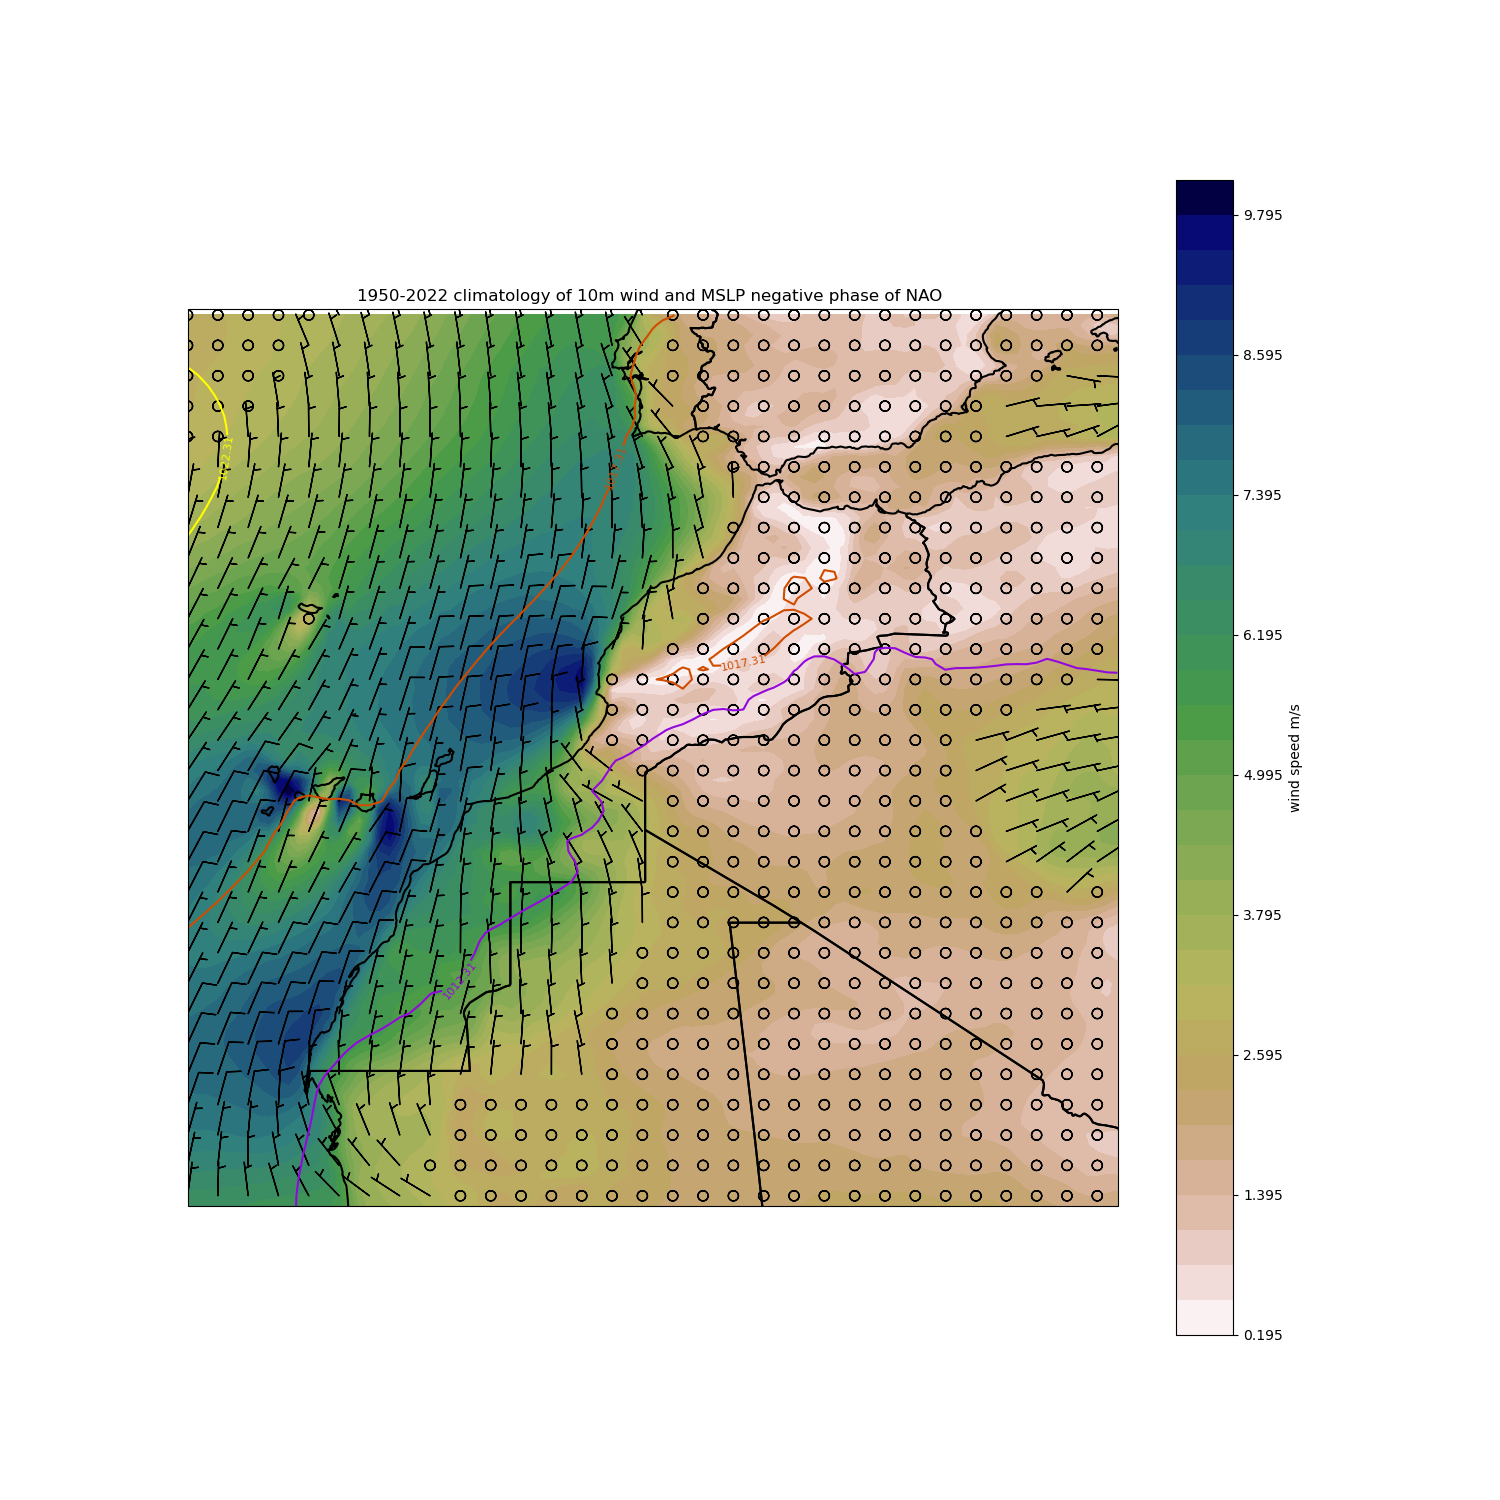
\includegraphics[scale=0.3]{NEG_PHASE.png}
\caption{Climatologie du vent et de la pression pour la phase NAO- (1950–2022).}
\label{fig:nao_negative}
\end{figure}

En revanche, la phase NAO- est caractérisée par des conditions favorables à l’upwelling :
\begin{itemize}
    \item \textbf{Direction du vent :} Les vents deviennent parallèles à la côte, favorisant un transport d'Ekman plus efficace. Cet alignement optimal est particulièrement marqué dans la région sud.
    \item \textbf{Intensité du vent :} Les vitesses moyennes atteignent environ 10 m/s, augmentant considérablement la dynamique de remontée des eaux froides.
    \item \textbf{Impact sur le CUI :} Une phase NAO- stimule fortement l’upwelling, renforçant la productivité biologique et soutenant les écosystèmes marins. Ces conditions sont idéales pour les activités de pêche dans la région.
\end{itemize}

\subsection{Discussion et implications}
Ces résultats démontrent que l'upwelling côtier au Maroc est influencé de manière significative par les phases de la NAO. La phase positive entraîne une diminution de l’upwelling, tandis que la phase négative l’intensifie. Ces variations impactent directement les écosystèmes marins et les activités économiques dépendantes, comme la pêche. Une analyse complémentaire, incluant des simulations climatiques futures, pourrait aider à anticiper les impacts du changement climatique sur cette dynamique essentielle.

\newpage
\section*{Acronymes}
\begin{tabular}{|l|p{8cm}|}
\hline
\textbf{Acronyme} & \textbf{Définition} \\
\hline
CUI               & Coastal Upwelling Index (Indice d'Upwelling Côtier) \\
NAO               & North Atlantic Oscillation (Oscillation Nord-Atlantique) \\
ERA5              & European Centre for Medium-Range Weather Forecasts Reanalysis 5 (Réanalyses ERA5) \\
NOAA              & National Oceanic and Atmospheric Administration \\
SST               & Sea Surface Temperature (Température de la Surface de la mer) \\
CDO               & Climate Data Operator \\
ERDDAP			   & Environmental Research Division's Data Access Program \\ 
\hline
\end{tabular}

\newpage

\section*{Références}
\begin{thebibliography}{99}
    \bibitem{BakunWeeks} Bakun, P., \& Weeks, S. J. (1995). Coastal Upwelling Indices, West Coast of North America, 1946-1995. \textit{NOAA Technical Report NMFS-SWFSC-231}.
    \bibitem{NOAA} NOAA. (2024). ERDDAP. \url{http://coastwatch.pfeg.noaa.gov/erddap/griddap/erdlasFnWPr.html}.
    \bibitem{ECMWF} European Centre for Medium-Range Weather Forecasts (ECMWF). (2024). ERA5 Reanalysis. \url{https://climate.copernicus.eu/climate-reanalysis}.
    \bibitem{HurrellDeser} Hurrell, J. W., \& Deser, C. (2009). North Atlantic climate variability: The role of the North Atlantic Oscillation. \textit{Journal of Marine Systems}, 78(1), 28-41.
    \bibitem{Trigo} Trigo, R. M., Osborn, T. J., \& Corte-Real, J. (2002). The North Atlantic Oscillation influence on Europe: Climate impacts and associated physical mechanisms. \textit{Climate Research}, 20(1), 9-17.
    \bibitem{Feddersen} Feddersen, H., et al. (2006). Influence of the NAO on Mediterranean precipitation and variability. \textit{Geophysical Research Letters}, 33(5).
    \bibitem{Santos} Santos, J. A., Corte-Real, J., \& Leite, S. M. (2005). Atmospheric large-scale dynamics during the 2004/2005 winter drought in Portugal. \textit{International Journal of Climatology}, 25(5), 581-601.
    \bibitem{Benazzouz} Benazzouz, A., \& Boudia, S. (2021). Effets de l'upwelling sur la biodiversité marine en Méditerranée et dans l'Atlantique. \textit{Journal of Marine Science}, 34(2), 157-164.
    \bibitem{Gomez} Gomez, P., \& Abid, A. (2020). Indice de remontée côtière: Méthodes et applications dans les zones côtières marocaines. \textit{Climate Research}, 52(3), 200-210.
    \bibitem{Hurrell95} Hurrell, J. W. (1995). Decadal trends in the North Atlantic Oscillation and relationships to regional temperature and precipitation. \textit{Science}, 269(5224), 676-679.
    \bibitem{Masson} Masson-Delmotte, V., et al. (2018). Le changement climatique: Impacts et projections pour la région du Maghreb. \textit{Global Change Research Journal}, 27(5), 97-105.
    \bibitem{Rodwell} Rodwell, M. J., \& Folland, C. K. (2002). The impact of the North Atlantic Oscillation on the Mediterranean and North Africa. \textit{Geophysical Research Letters}, 29(8), 113-118.
    \bibitem{Albouy} Albouy, C., \& Leprieur, F. (2015). Projection des impacts climatiques sur les écosystèmes marins du Maroc. \textit{Climate and Ecosystem Dynamics}, 48(2), 32-45.
    \bibitem{Bensalem} Bensalem, M., \& El Hadj, A. (2019). Temporal variations of coastal upwelling along the Moroccan Atlantic coast. \textit{Oceanography Studies}, 29(4), 213-230.
    \bibitem{IPCC} IPCC. (2014). Rapport spécial sur le changement climatique: Impacts, adaptation et vulnérabilité. \textit{Intergovernmental Panel on Climate Change}, 121-157.
\end{thebibliography}

\newpage
% Ajouter une image en illustration

\listoffigures
\newpage



\end{document}
